\documentclass[11pt]{article}
\usepackage{fullpage,url}
\usepackage{amsmath,amsthm,amssymb}
\usepackage{graphicx}
\usepackage{eso-pic}
\usepackage{bm}
\usepackage{caption}
\usepackage{picins}   
\usepackage{microtype}
\usepackage{multirow}
\usepackage{url}
\usepackage{enumerate}
\usepackage{pdfpages}
\usepackage{fancyvrb}
\usepackage[letterpaper,top=1in,bottom=1in,left=1in,right=1in,nohead]{geometry}

\newcommand{\PhiB}{\mathbf{\Phi}}
\newcommand{\Ll}{\mathcal{L}}
\newcommand{\Nn}{\mathcal{N}}
\newcommand{\Uu}{\mathcal{U}}
\newcommand{\Ee}{\mathcal{E}}
\newcommand{\Aa}{\mathcal{A}}
\newcommand{\Hh}{\mathcal{H}}
\newcommand{\Ii}{\mathcal{I}}
\newcommand{\Ff}{\mathcal{F}}
\newcommand{\Dd}{\mathcal{D}}
\newcommand{\Tt}{\mathcal{T}}
\newcommand{\Pp}{\mathcal{P}}
\newcommand{\Ss}{\mathcal{S}}
\newcommand{\Cc}{\mathcal{C}}
\newcommand{\Oo}{\mathcal{O}}
\newcommand{\Bb}{\mathcal{B}}
\newcommand{\Rr}{\mathcal{R}}
\newcommand{\Rm}{\mathrm{R}}
\newcommand{\CB}{\mathbf{C}}
\newcommand{\RB}{\mathbf{R}}
\newcommand{\xB}{\mathbf{x}}
\newcommand{\yB}{\mathbf{y}}
\newcommand{\XB}{\mathbf{X}}
\newcommand{\YB}{\mathbf{Y}}
\newcommand{\fB}{\mathbf{f}}
\newcommand{\ZB}{\mathbf{Z}}
\newcommand{\SB}{\mathbf{S}}
\newcommand{\AB}{\mathbf{A}}
\newcommand{\WB}{\mathbf{W}}
\newcommand{\TB}{\mathbf{T}}

\newcommand{\omitme}[1]{}
\newtheorem*{lemma}{Lemma}
\newtheorem{case}{Case}

\makeatletter
\newcommand{\specialnumber}[1]{%
  \def\tagform@##1{\maketag@@@{(\ignorespaces##1\unskip\@@italiccorr#1)}}%
}

\setlength{\parindent}{0in}
\setlength{\parskip}{6pt}

\DeclareMathOperator{\E}{E}
\DeclareMathOperator{\Var}{Var}
\DeclareMathOperator{\Unif}{Unif}

\begin{document}
\thispagestyle{empty}
{\large{\bf CS7640: Advanced Image Processing \hfill Prateep Mukherjee(u0876583)}}\\

{\LARGE{\bf Homework 1}}
\vspace{0.2\baselineskip}
\hrule

\section{Introduction}
\label{sec1}

\par In this project we explore the application of image denoising using total variation. We implement the algorithm explained in \cite{Chambolle}, which is a faster version of the method developed by Rudin et al. \cite{Rudin}. As discussed in class, we use the dual formulation of the objective. This method is emperically faster and solves the denosing problem effectively. For comparison, we use the non-linear denoising algorithm proposed by \cite{Malik}. 

\par The following sections present details of the steps discussed in the above papers, and also provides information about the implementation choices made. Section \ref{sec2} describes the notations involved in the algorithm. 

\section{Notations}
\label{sec2}

Our images will be 2-dimensional matrices of size $N \times N$. Let us denote by $\Omega$ the Euclidean space $\Re^{N \times N}$. To define the discrete total variation, we define a discrete gradient operator. If $u \in \Omega$, the gradient $\nabla x$ is a vector in $Y := \Omega \times \Omega$ given by :
\vspace{-5pt}
\begin{equation*}
  (\nabla u)_{i,j} = ( (\nabla u)^{1}_{i,j}, (\nabla u)^{2}_{i,j}) 
\end{equation*}

with,
\vspace{-5pt}
\begin{eqnarray*} 
	(\nabla u)^{1}_{i,j} = 
	\begin{cases}
		u_{i+1,j} - u_{i,j}, & \ \mbox{$i < N$}, \\
		0, & \mbox{if $i = N$}
	\end{cases} \\
	(\nabla u)^{2}_{i,j} = 
	\begin{cases}
		u_{i,j+1} - u_{i,j}, & \ \mbox{$j < N$}, \\
		0, & \mbox{if $j = N$}
	\end{cases}
\end{eqnarray*}

for $i,j = 1, \cdots, N$. The total variation of $u$ is defined by
\vspace{-5pt}
\begin{equation*}
J(u)  = \sum\limits_{1 \le i,j \le N} | (\nabla u)_{i,j} |,
\end{equation*}
with $|y| := \sqrt{y_{1}^2 + y_{2}^2}$ for every $y = (y_1, y_2) \in \Re^2$.

\par The idea is to replace the optimization of the image $\Omega$ by the optimization of the vector field $G$ that is related to $\Omega$ by $f = y - \lambda \; div \; G$, subject to constraints that $\forall x \in \Omega,  \| G_x\| \le 1$.

\par Chambolle proposed an algorithm for solving 
\vspace{-5pt}
\begin{equation}
 \min\limits_{x \in \Omega} \frac{ \| u - g\|^2 }{2\lambda} + J(u),
 \label{eq1}
\end{equation}

given the observed image $g \in \Omega$ and $\lambda > 0$. The Euler equation for Eq. \ref{eq1} is 
\vspace{-5pt}
\begin{equation*}
u - g + \lambda \partial J(u) = 0
\end{equation*}

Computing the nonlinear projection $\pi_{\lambda K}(g)$ amounts to solving the corresponding dual problem:
\vspace{-5pt}
\begin{eqnarray}
  \min\limits_{p \in Y} \| \lambda \; div \; p - g\|^2 \\
    |p_{i,j}|^2 \le 1, \: \: \forall i,j = 1, \cdots N \notag
 \label{eq2}
\end{eqnarray}

The Karush-Kuhn-Tucker(KKT) conditions yield the existence of a Lagrange multiplier $\alpha_{i,j} \ge 0$, associated to each constraint in Eq. \ref{eq2}, such that 
\vspace{-5pt}
\begin{equation*}
-(\nabla(\lambda \; div \; p - g))_{i,j} + \alpha_{i,j} p_{i,j} = 0, \: \: \forall (i,j) \in \Omega
\end{equation*}

with either $\alpha_{i,j} > 0$ and $p_{i,j} = 1$, or $\alpha_{i,j} = 0$ and $|p_{i,j}| < 1$. In the latter case, also $(\nabla(\lambda \; div \; p - g))_{i,j} = 0$. Therefpre, $\alpha_{i,j} = |((\nabla(\lambda \; div \; p - g))_{i,j}|$. The iterative solution is formulated as:
\vspace{-5pt}
\begin{eqnarray*}
  p_{i,j}^{n+1} = & p_{i,j}^n + \tau [ (\nabla(div \; p^{n} - \frac{g}{\lambda}))_{i,j}  \\
  		& -|(\nabla(div \; p^{n} - \frac{g}{\lambda}))_{i,j}| p_{i,j}^{n+1} ],
\end{eqnarray*}
Therefore,
\begin{equation}
p_{i,j}^{n+1} = \frac{p_{i,j}^{n} + \tau (\nabla(div \; p^{n} - \frac{g}{\lambda}))_{i,j} }{ 1 +  |(\nabla(div \; p^{n} - \frac{g}{\lambda}))_{i,j}| }
\label{eq3}
\end{equation}
\vspace{-5pt}
Next, the author shows that as $n \rightarrow \infty$, if $\tau \le 1/8$, $\lambda \; div \; p^{n}$ converges to $\pi_{\lambda K}(g)$.

\vspace{-10pt}
\section{Algorithm}
\label{sec3}
\vspace{-10pt}

As described in section \ref{sec2}, we are solving the following objective:
\vspace{-5pt}
\begin{equation}
	\min\{J(u) : \| u - g \|^2 = N^2\sigma^2\}
\vspace{-5pt}
\label{eq4}
\end{equation}

where $N^2$ is the total number of pixels. Chambolle proposed the following algorithm in order to solve Eq. \ref{eq4}. Assume $N\sigma \in [0, \| g - \bar{g}\|]$, where $\bar{g}$ is the average value of the pixels $g_{i,j}$. We need to find a value $\bar{\lambda}$ for which $f(\bar{\lambda}) = N\sigma$. We choose a random initial value $\lambda_{0} > 0$, and compute $v_0 = \pi_{\lambda_0 K}(g)$ and $f_0 = f(\lambda_0) = \| v_0\| $.

\vspace{-10pt}
\section{Results}
\label{sec4}
\vspace{-10pt}
\begin{figure}[!hbt]
\vspace{-10pt}
  \begin{center}
  \[\begin{array}{cccc}
  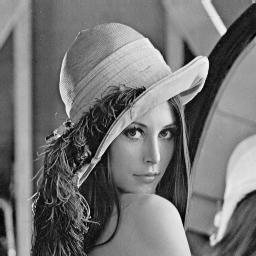
\includegraphics[width=0.33\linewidth] {tv_orig.png} &
   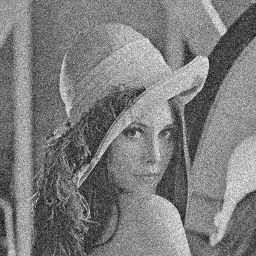
\includegraphics[width=0.33\linewidth] {tv_noise.png} &
   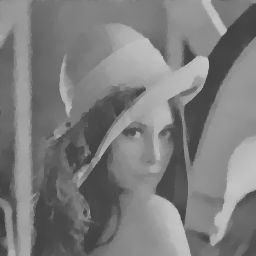
\includegraphics[width=0.33\linewidth] {tv_denoise.png} \\
 (a) & (b) & (c) \\
  \end{array}\]
\end{center}
\vspace{-15pt}
\caption{{\bf Lena:} (a) Original image($g$); (b) Original image with added noise($u$) with $\sigma = 0.1$; (c) Denoised image using Chambolle's algorithm
}
\label{fig1}
\end{figure}

\vspace{-10pt}
\begin{figure}[h]
\vspace{-10pt}
  \begin{center}
  \[\begin{array}{cccc}
  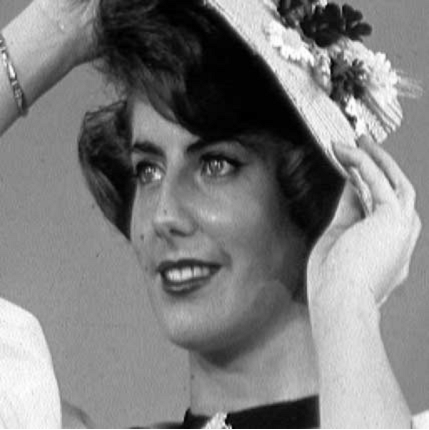
\includegraphics[width=0.33\linewidth] {img1_orig.png} &
   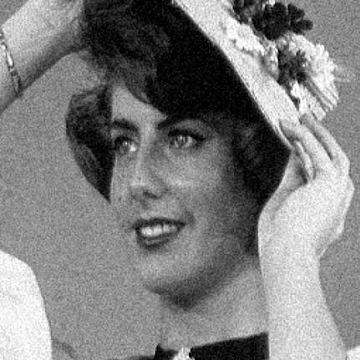
\includegraphics[width=0.33\linewidth] {img1_sigma_12.png} &
   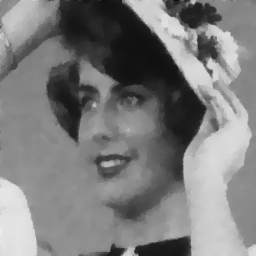
\includegraphics[width=0.33\linewidth] {tv_denoise_1.png} \\
 (a) & (b) & (c) \\
  \end{array}\]
\end{center}
\vspace{-15pt}
\caption{(a) Original image($g$); (b) Original image with added noise($u$) with $\sigma = 12$; (c) Denoised image using Chambolle's algorithm
}
\label{fig2}
\end{figure}

Fig. \ref{fig1} shows performance of Chambolle's algorithm on the classical "lena" image, corrupted with Gaussian noise of $\sigma = 0.1$.  The original is a $256 \times 256$ square image with intensity values ranging from 0 to 255. The original algorithm is modified slightly in that we perform a nested loop of iterations, where the inner loop iteratively solves eq. \ref{eq3} until convergence is reached. The outer loop feeds the corrected image for one pass of the algorithm as input(or, observed) image to the next pass. For attaining the output shown in Fig. \ref{fig1}, we perform 100 iterations(inner loop) of solving Eq. \ref{eq3} and 50 passes(outer loop) of the algorithm. The other parameters were set as follows: $\tau = 0.25$, $\lambda = 0.5$. The dual variable $p$ was initialized to a blank image of same size as $g$.

Fig. \ref{fig2} shows another example of Chambolle's algorithm. Here, the original image was corrupted with noise of standard deviation $\sigma = 12$. The same number of inner and outer-loop iterations were required for denoising this. 


\clearpage
\begin{thebibliography}{9}
\vspace{-9pt}

\bibliographystyle{IEEEbib}
\small  % Use 9 point text.
\addtolength{\itemsep}{-8pt}

\bibitem{Chambolle}
A. Chambolle, `An Algorithm for Total Variation Minimization and Applications,` \emph{Journal of Mathematical Imaging and Vision}, pp. 89-97, 2004. 

\bibitem{Rudin}
I. Rudin, S. Osher, Stanley and E. Fatemi, `Nonlinear Total Variation Based Noise Removal Algorithms,`, \emph{Phys. D}, pp 259--268, 1992.

\bibitem{Malik}
P. Perona, and J. Malik, `Scale-Space and Edge Detection Using Anisotropic Diffusion`, \emph{IEEE PAMI}, vol. 12, no. 7, 1990.
\end{thebibliography}

\end{document}